\documentclass[11pt]{article}

\usepackage[margin=1.1in]{geometry}
\usepackage{booktabs}
\usepackage{amsmath}
\usepackage{graphicx}
\usepackage[colorlinks=true,linkcolor=black,urlcolor=blue,citecolor=black]{hyperref}
\usepackage{caption}
\graphicspath{{../artifacts/plots/}}

\title{Does draft-order modeling beat expert consensus?\\
\large A counterfactual evaluation of five drafting policies}
\author{Yousuf Rashid\\ \small University of Waterloo}
\date{}

\begin{document}
\maketitle

\begin{abstract}
\noindent
I built a system to pick fantasy basketball players better than the default
rankings do. It has three parts: an XGBoost projection model, a Cox
proportional-hazards model for when each player comes off the board, and a Monte
Carlo layer that uses the second to decide how to spend the first. Then I tested
the whole thing against the ranking it was supposed to beat, over 4{,}400
replayed drafts.

It lost. Average draft position (ADP) predicts realized production better than
anything I fit ($\rho = 0.574$ against $0.555$ for my value estimate and $0.529$
after a positional adjustment), and every policy built on those estimates
finished behind the policy that just follows ADP. The survival model itself is
accurate, with concordance $0.935$ and expected calibration error $0.029$.
Knowing when a player comes off the board just does not improve the pick.

The interesting part is how the answer changed with sample size. At 132 paired
drafts the sequencing policy looked like it won by $+2.35$ points. At 1{,}056 the
edge was $-0.14$ and it lost 54\% of head-to-head drafts. The first number was
noise, and I would have reported it if I had stopped there.
\end{abstract}

\section{What the system does}

A snake draft has a structure that rewards thinking ahead. You pick at 6, then
not again until 19, then 30. Thirteen players leave the board between your turns.
If you want two of them, the order you take them in matters: take the one who
will still be there later, and you lose him.

That is the whole idea. Formally, at pick $j$ with a next turn at $k$, the value
of waiting on player $i$ depends on
\[
P(\text{available at } k \mid \text{available at } j)
= \frac{S_i(k)}{S_i(j)},
\]
the conditional survival ratio rather than $S_i(k)$ on its own. The distinction
matters more than it looks. A player with an ADP of 5 who is somehow still on the
board at pick 20 is a different proposition from the same player before the draft
started, and only the ratio knows that.

Three models feed the decision.

\paragraph{Projections (Model A).}
XGBoost per category, trained on season-to-season transitions with lag features,
age, and team-context terms. Rookies have no history to lag, so they shrink
toward a prior fit on what players from the same draft-pick tier actually did,
weighted $w = n/(n+k)$ on career minutes.

\paragraph{Availability (Model B).}
A Cox proportional-hazards model over draft durations, with Kaplan--Meier curves
as the non-parametric fallback. Held-out concordance is $0.935$; expected
calibration error is $0.029$, which matters because the decision layer consumes
the probability, not the ranking.

\paragraph{Games played.}
Added after the first backtest, and the one place a model clearly helped. The
projection code multiplied every per-minute rate by a flat 82 games, so it assumed
everyone plays a full season. League-average games played is about 46. A
games-played model cut RMSE from $38.3$ to $18.5$, a 52\% reduction against the
flat assumption and 19\% against repeating last season's total.

\section{The backtest}

This is counterfactual policy evaluation: estimating what a policy would have
earned on data generated by a different policy. My agent drafts from one slot
using the policy under test. The other teams draft from that season's actual ADP
board, jittered per seed so the opponents are not identical every run. Rosters are
scored on \emph{realized} end-of-season production, not on projections. Score
on projections and a policy can win by agreeing with its own model.

\begin{table}[h]
\centering
\caption{Sweep dimensions. Every comparison is paired on
(season, league size, slot, seed), so the draft's own luck cancels.}
\begin{tabular}{ll}
\toprule
Seasons & 2020--21 through 2025--26 (6) \\
League sizes & 10 and 12 teams \\
Draft slots & all, exhaustively \\
Seeds & 8 per configuration \\
Rollout simulations & 60 per candidate \\
Total drafts & 4{,}400 \\
\bottomrule
\end{tabular}
\end{table}

Roster legality lives inside the rollout rather than in a separate optimizer.
Starting slots (4G/4F/2C) fill before the three bench seats, so the bench is the
slack that absorbs a positional run. A draft that returns 12 or 14 players is a
bug, and the harness asserts against it.

Two details cost me real time. Simulating to the end of the draft was wasted work,
since picks after your last one cannot change your roster; stopping there was
the single largest speedup. And scoring every candidate against \emph{common
random numbers}, meaning the same opponent draws, made the argmax stable at 60
simulations instead of the 1{,}000 I had budgeted. I checked 30 and it was not
enough: only one of three draft states gave a stable answer across seeds.

\section{The ablation ladder}

Five policies, one harness. Rungs 0 through 3 see identical inputs, so any
difference between them is the decision rule and nothing else. Only rung 4 swaps
in my own projections, which is what makes rung 4 minus rung 3 a separate
measurement of whether the projection model was worth anything.

\begin{table}[h]
\centering
\caption{Realized starter value, 1{,}056 paired drafts per rung
(176 for rung 4, which needs projections and so runs on 2025--26 only).
Win rate is against the rung below.}
\begin{tabular}{clrrrc}
\toprule
Rung & Policy & {Mean} & {Edge} & {Win rate} & 90\% interval \\
\midrule
0 & Follow ADP & 61.50 & -- & -- & -- \\
1 & Best available by value    & 60.21 & -1.29  & 0.375 & $[-14.0, +10.7]$ \\
2 & VORP, greedy               & 54.22 & -5.99  & 0.293 & $[-26.2, +14.7]$ \\
3 & VORP $+$ sequencing        & 54.07 & -0.14  & 0.457 & $[-14.2, +14.6]$ \\
4 & Own projections $+$ both   &  3.76 & -46.32 & 0.023 & $[-73.7, -11.0]$ \\
\bottomrule
\end{tabular}
\end{table}

\begin{figure}[h]
\centering
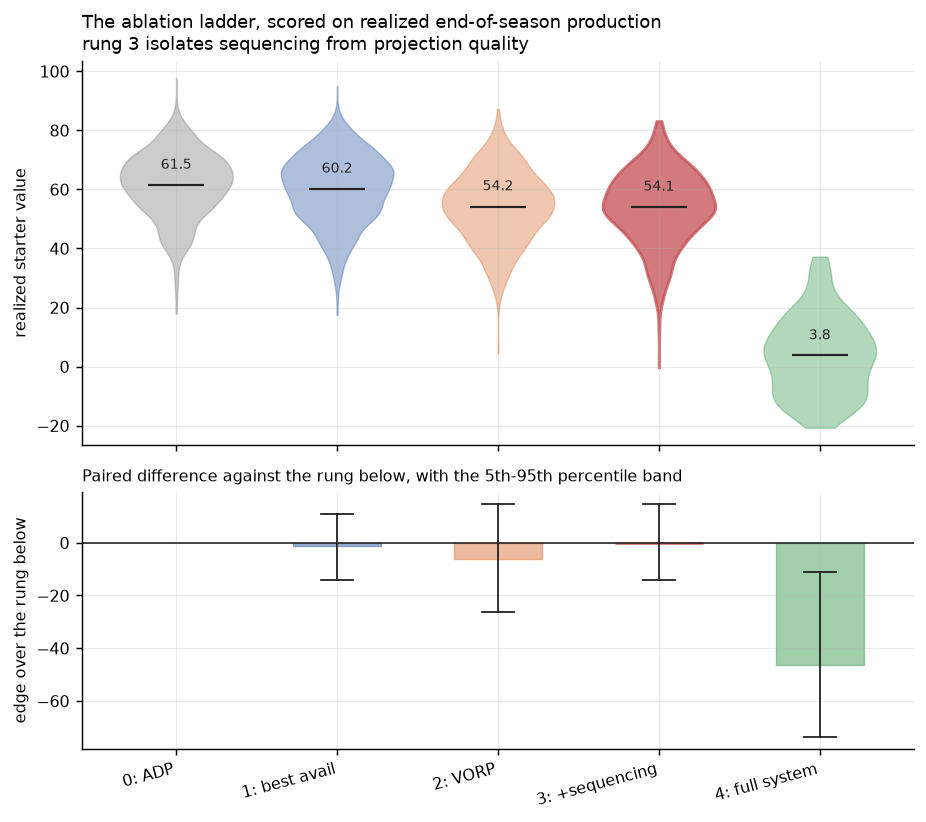
\includegraphics[width=\textwidth]{ladder.png}
\caption{The ladder as distributions rather than means. The violins are realized
starter value across all 1{,}056 paired drafts per rung; the lower panel is the
paired difference against the rung below with its 5th--95th percentile band. Every
band except rung 4's contains zero, which is the shape of the whole result: the
losses are real but small against the draft's own variance.}
\label{fig:ladder}
\end{figure}

Rung 3 is the comparison the design exists for. It holds projections fixed
against rung 2 and changes only whether the policy simulates forward, so it
isolates sequencing from projection quality. The answer is $-0.14$ points and a
45.7\% win rate. Sequencing does not help. Figure~\ref{fig:ladder} shows why the
means alone understate how little separates the rungs: the distributions overlap
almost entirely.

Against ADP directly, rung 3 wins 25.6\% of paired drafts and zero of twelve
draft slots. It is not that sequencing works from some positions and not others.
It loses everywhere. Figure~\ref{fig:sequencing} is the same comparison
per draft rather than in aggregate.

\begin{figure}[h]
\centering
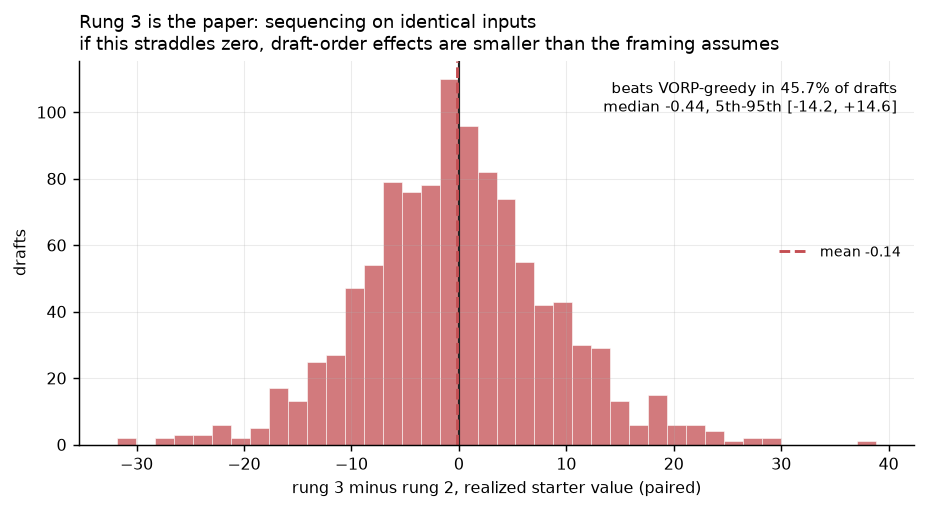
\includegraphics[width=0.95\textwidth]{sequencing_effect.png}
\caption{Sequencing on identical inputs, draft by draft. If simulating the board
forward helped, this would sit to the right of zero. It is centred on it, with a
median of $-0.44$ and a 5th--95th range of $[-14.2, +14.6]$: the per-draft spread is
two orders of magnitude wider than the effect being measured.}
\label{fig:sequencing}
\end{figure}

\subsection{The result I nearly published}

My first run used one season, two league sizes, and six seeds: 132 paired drafts.
Rung 3 beat rung 2 by $+2.35$ with a 55.3\% win rate, and the per-combination
numbers pointed the same way both times. I wrote it down as ``directionally
consistent.''

It was not. The 90\% interval on that estimate was $[-16.3, +25.3]$, roughly ten
times wider than the effect. At eight times the sample the edge collapsed to
$-0.14$. Nothing about the model changed between those two runs.

I am putting this in the paper because the interval was visible the whole time and
I still described a coin flip as a direction. If the sweep had stopped at 132
drafts, the writeup would have claimed a win.

\section{Why every learned policy lost}

A negative result is only useful with a diagnosis, so I tested each value estimate
directly against realized production. Rank correlation, six seasons, higher is
better.

\begin{figure}[h]
\centering
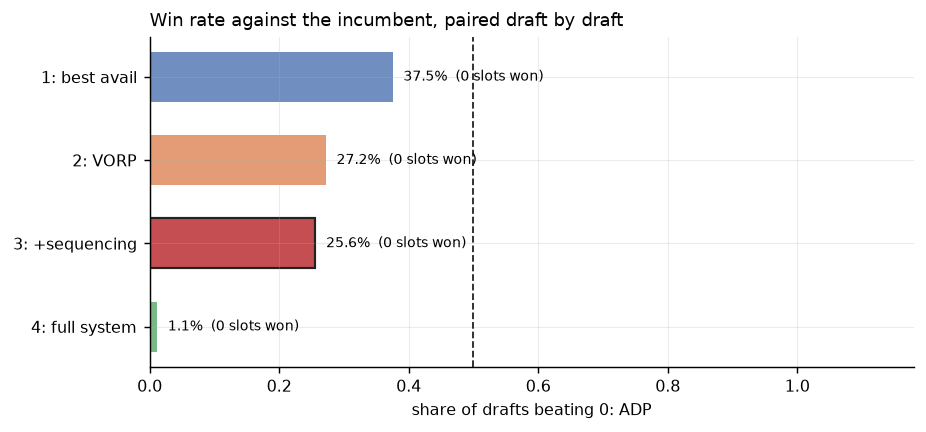
\includegraphics[width=0.86\textwidth]{win_rates.png}
\caption{Share of paired drafts each policy wins against the incumbent. A policy
that merely had higher variance would sit near 50\%; every rung sits below it.}
\label{fig:winrates}
\end{figure}

\begin{figure}[h]
\centering
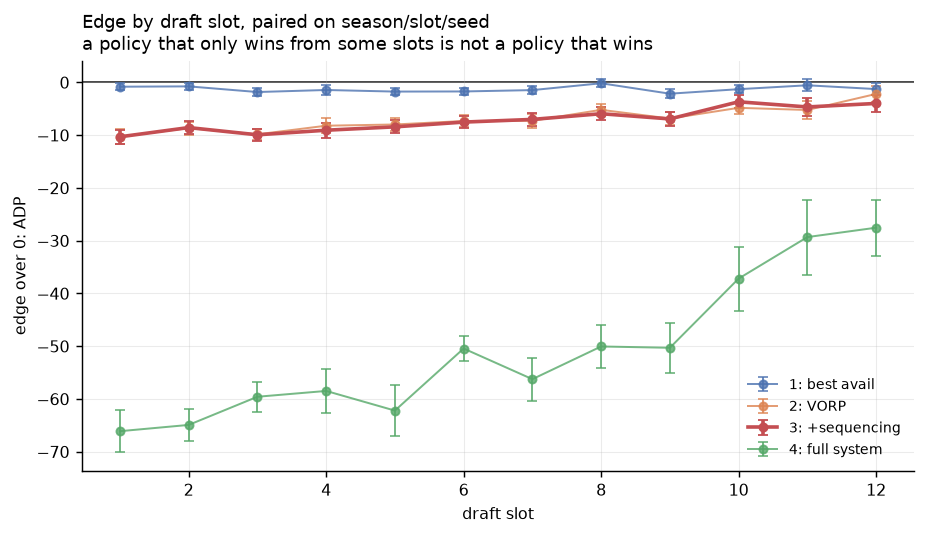
\includegraphics[width=\textwidth]{by_slot.png}
\caption{Edge over ADP by draft slot. Sequencing should pay most from the turn
ends, where the wait between picks is longest, and it does not pay anywhere: rung 3
loses at all twelve slots. A policy that worked from some positions and not others
would show a slope here.}
\label{fig:byslot}
\end{figure}

\begin{table}[h]
\centering
\caption{How well each ranker predicts realized value (Spearman $\rho$).}
\begin{tabular}{lrr}
\toprule
Ranker & {Full board} & {Top 60} \\
\midrule
ADP rank                  & 0.574 & 0.368 \\
Board-implied value       & 0.555 & 0.360 \\
Value over replacement    & 0.529 & 0.316 \\
Own projections           & 0.331 & 0.270 \\
\bottomrule
\end{tabular}
\end{table}

ADP wins on the full board and again in the top 60, where drafts are actually
decided, and Figures~\ref{fig:winrates} and~\ref{fig:byslot} show the consequence
draft by draft and slot by slot. So rungs 1 through 4 are not losing because the decision layer is
broken. They are optimizing a worse objective than the ranking they are trying to
beat, and no amount of sequencing fixes an inferior input. Rung 3 was doing
competent inference on the wrong numbers.

This is a market-efficiency finding, and in hindsight it should have been the
prior. ADP is a consensus of experts who update daily on injury news, minutes
expectations, and beat reporting. My projections see prior-season box scores.
When those two disagree, the box scores are usually the ones missing something.

\subsection{Where the result does and does not hold}

The finding survives both cuts of the sweep. Splitting by season checks that no
single year is carrying it, and splitting by league size checks the mechanism: a
deeper board means longer waits between picks, so if sequencing worked at all it
should work best in the smallest league.

\begin{figure}[h]
\centering
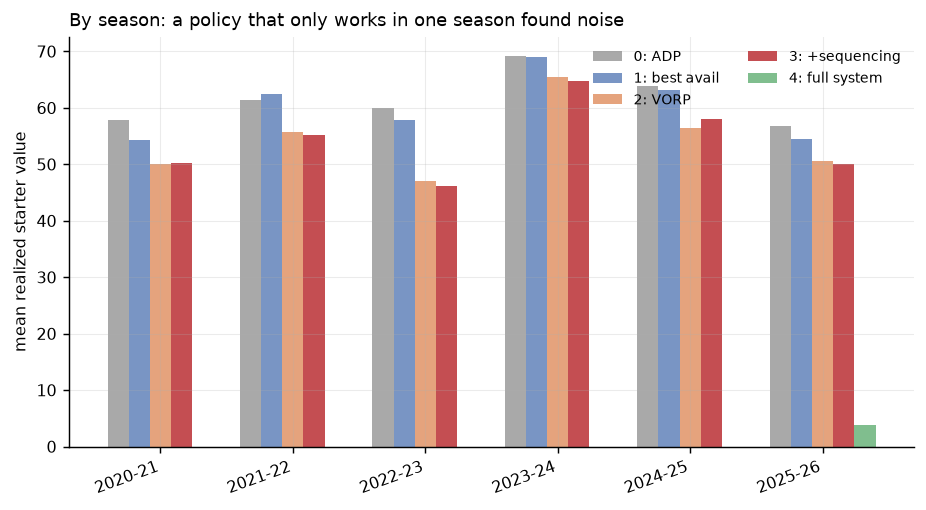
\includegraphics[width=\textwidth]{by_season.png}
\caption{Mean realized starter value by season. The rung ordering is stable across
all six, so the result is not one season's injuries. Absolute values move a lot
between seasons, which is why every comparison in this paper is paired.}
\label{fig:byseason}
\end{figure}

\begin{figure}[h]
\centering
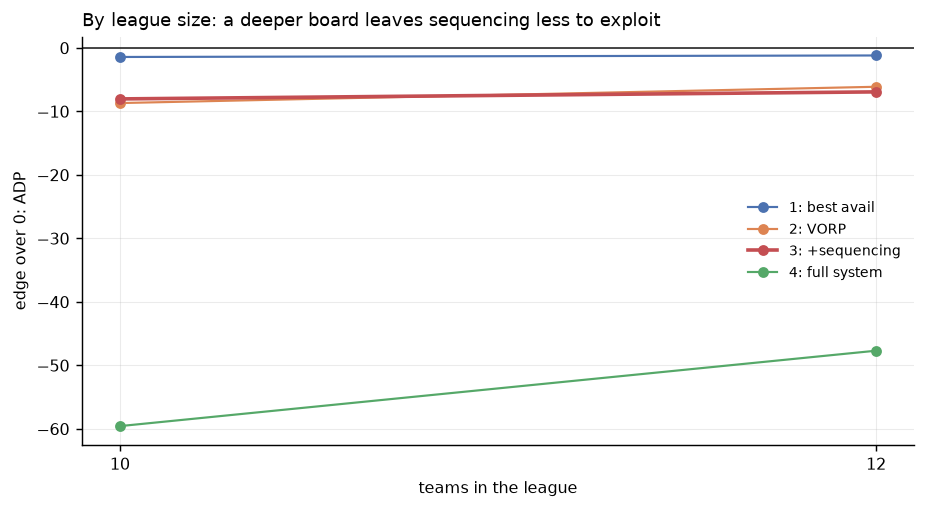
\includegraphics[width=0.9\textwidth]{by_league_size.png}
\caption{Edge over ADP by league size. Ten and twelve teams give the same answer.
The mechanism predicted a gradient here and there is not one.}
\label{fig:byleaguesize}
\end{figure}

\subsection{One correction to the table}

Rung 2's $-5.99$ overstates its failure, and the cause is my scoring. The ladder
above scores starters only. VORP-greedy drafts depth on purpose and strands $9.23$
points on the bench, against $5.05$ for ADP. Scored on total roster value the
penalty falls to $-2.10$ and its win rate rises from 29\% to 44\%.

Rung 3 stays negative under both metrics ($-0.14$ starters, $-2.48$ total), so the
sequencing conclusion holds either way. But the honest statement about rung 2 is
that a chunk of its deficit was a choice I made about scoring, not something the
policy did.

\subsection{What the projection model was worth}

Rung 4 is the weakest rung at $3.76$, and most of that traces to one thing the
data cannot supply. Four players (VanVleet, Lillard, Irving, Haliburton)
were projected for 61 to 66 games and played zero. All four were ruled out after
the ADP board published.

No feature built from prior-season statistics can know that. A live injury feed
could, and the database has no historical one: \texttt{player\_status} is a single
snapshot with no per-season history, so a past draft's injury designations cannot
be reconstructed. Reading today's status onto a 2018 row would leak the future,
since today's status partly reflects what happened after that draft.

So the games-played model corrects the population-level bias, which was real and
large, and cannot correct individual unforeseeable injuries. I am not going to
pretend otherwise by fitting something that appears to predict them. The ADP board
handles these cases and my model does not, and that gap is a large part of why
rung 4 finishes where it does.

\section{A data bug worth recording}

Partway through the diagnosis, VORP-greedy was drafting players with high value
and zero realized production. Four of them on the 2025--26 board had no position
at all.

The ADP ingest normalized names by stripping generational suffixes before
matching, so ``Jaren Jackson Jr.'' collapsed onto ``Jaren Jackson.'' The lookup
kept the lowest player id, which is the father. Seven players were linked to their
fathers across all twelve seasons: Jackson, Hardaway, Nance, Porter, Trent, Smith,
Payton. The fathers have no current roster row and no current statistics, so those
players became position-less entries worth nothing, which is worse than being
unmatched because they still carried an inflated VORP.

The fix matches on the exact name first and falls back to the suffix-stripped form
only when no player claims the exact one. Suffix-stripping still has to exist, because
``Russell Westbrook III'' and ``Russell Westbrook'' are the same man, so the
fallback map refuses to answer when two real players share a base name. Seven
links corrected, no regressions, and the same five unmatched names as before, all
of whom never played an NBA game.

This is the same failure mode the project had already hit and fixed for accented
names, where Joki\'c and Don\v{c}i\'c silently failed to link. Suffixes were the
case that got missed.

\section{What I would do next}

Not more sequencing. The survival model works and the decision layer works; the
inputs are the problem, and the diagnosis says ADP already contains what my
projections estimate. Beating it needs signal ADP does not have. A live
injury feed is the obvious candidate, since that is the one gap I can point at
with a number attached.

The part I would keep is the harness. Four thousand paired off-policy drafts with
per-slot and per-seed distributions is the machinery that told me the $+2.35$ was
noise, and it would have told me the same thing about any other idea I tried.

\section*{Reproducing this}

\begin{itemize}\itemsep2pt
\item \texttt{models/projection/} --- XGBoost projections, games-played model,
      rookie priors, walk-forward validation.
\item \texttt{models/behaviour/} --- Kaplan--Meier and Cox survival models,
      calibration, and the availability query the rollout calls.
\item \texttt{models/decision/} --- rollout, the five policies, the backtest
      harness, plots.
\item \texttt{artifacts/backtest.csv} --- all 4{,}400 drafts, one row each.
\item \texttt{artifacts/ablation\_ladder.csv} --- the ladder table.

\item \texttt{tests/} --- 141 tests. The 70 that need no database run in CI on
      every push; the rest skip, since the database is published as a release
      asset rather than committed.
\end{itemize}

Every module also runs standalone as a worked example. Splits are temporal
everywhere: a draft is a point in time, and training on 2025 to predict 2019 would
be a leak that reports a better number for itself. Leak detection is a gate rather
than only a test --- the rate trainer refuses to run if it fires, and beyond
checking feature names it permutes the current season's statistics and rebuilds,
since a feature whose value moves was reading the season it is meant to predict.

\end{document}
